\section{Laboratory Measurements of Sulfur Dioxide}

Verifying millimeter-wavelength absorption spectrum of SO$_2$ is important for the study of the atmosphere of Venus. Making measurements under simulated Venus conditions assures the accuracy of any model derived from such measurements.
 Described below is the theory, laboratory equipment, measurement procedure and derived uncertainties in the measurements of the millimeter-wavelength absorptivity of gaseous sulfur dioxide under simulated Venus conditions.

\subsection{Measurement Theory}

In this experimental program, quality factor (Q) of a resonant mode of a resonator is used to measure the absorption of a gas or gas mixture \cite{high-sensitivity}. The quality factor of a resonance is given by \cite{matching}

\begin{equation} \label{eq:qlong}
Q = \frac{2\pi f_0 \textnormal{ x Energy Stored}}{\textnormal{Average Power Loss}}
\end{equation}

\noindent where $f_0$ is the resonant frequency. The Q of a resonance can be measured directly from $f_0$ by dividing it by its half-power bandwidth (HPBW).

\begin{equation} \label{eq:qshort}
Q = \frac{f_0}{HPBW}
\end{equation}

\noindent The Q of a lossy gas ($\epsilon'/\epsilon''$) and its opacity are related by
\begin{equation} \label{eq:alphaapprox}
\alpha \approx \frac{\epsilon'' \pi}{\epsilon' \lambda} = \frac{1}{Q_{gas}} \frac{\pi}{\lambda}
\end{equation}

\noindent where $\epsilon'$ and $\epsilon''$ are the real and imaginary permittivity of the gas, $\lambda$ is the wavelength in km, and $\alpha$ is the absoptivity of the gas in Nepers/km (1 Neper = 8.686 dB). Since Q can be affected by more than just the gas added, the Q of the gas-filled resonator is given by

\begin{equation} \label{eq:qloaded}
\frac{1}{Q_{loaded}^m} = \frac{1}{Q_{gas}} + \frac{1}{Q_{r}} + \frac{1}{Q_{ext1}} +\frac{1}{Q_{ext2}}
\end{equation}

\noindent where $Q_{loaded}^m$ is the measured quality factor of a resonance in the presence of a test gas, $Q_{gas}$ is the quality factor of the gas under test, $Q_{r}$ is the quality factor of the resonator in the absense of coupling losses, and $Q_{ext1}$ and $Q_{ext2}$ are the external coupling losses. Since the resonator used is symmetric, it is safe to assume $Q_{ext1} = Q_{ext2}$. Coupling losses can be derived from the transmissivity $t = 10^{-S/10}$, where $S$ is the measured insertion loss of the resonator in decibels (dB) at the frequency of a particular resonance using the following relationship

\begin{equation} \label{eq:t}
t = \left[ w \frac{Q^m}{Q_{ext}} \right]^2,
\end{equation}

\begin{equation} \label{eq:qext}
Q_{ext} = \frac{2Q^m}{\sqrt{t}}
\end{equation}

\noindent $Q_r$ is related to the measured Q at a vacuum by

\begin{equation}\label{eq:qvac}
\frac{1}{Q_{vac}^m} =  \frac{1}{Q_{r}} + \frac{1}{Q_{ext1}} +\frac{1}{Q_{ext2}}
\end{equation}

\noindent where $Q_{vac}^m$ is the measured Q at a vacuum. Substituting equation \ref{eq:qext} into equations \ref{eq:qloaded} and \ref{eq:qvac} gives

\begin{equation}\label{eq:qgas}
\frac{1}{Q_{gas}} = \frac{1 - \sqrt{t_{loaded}}}{Q^m_{loaded}} - \frac{1-\sqrt{t_{vac}}}{Q_{vac}^m}
\end{equation}

\noindent where $t_{loaded}$ and $t_{vac}$ are the transmissivity of the resonance taken in loaded and vacuum conditions respectively. When gas is added to the resonator there is a shift in the center frequency corresponding to the refractive index of the test gas. Since the quality factor is reliant on the center frequency this will affect the comparison between the two measurements. This effect is called dielectric loading \cite{h2s-labmesurements}. Dielectric matching can be achieved by performing additional measurements of the quality factor with a lossless gas present. Adding the lossless gas shifts the center frequency of the resonances, and by adding more or less gas the center frequency can be adjusted to be exactly the same as the lossy gas. These measurements are used in place of the vacuum measurements in equation \ref{eq:qgas} and by converting Nepers/km to dB/km we can rewrite equation \ref{eq:alphaapprox} as

\begin{equation} \label{eq:alphamatch}
\alpha = 8.686 \frac{\pi}{\lambda}\left(\frac{1 - \sqrt{t_{loaded)}}}{Q^m_{loaded}} - \frac{1-\sqrt{t_{matched}}}{Q_{matched}^m} \right) dB/km
\end{equation}

\subsection{Millimeter-Wavelength Measurement System}

The high-sensitivity millimeter-wavelength system used for measuring the opacity of gaseous sulfur dioxide under Venus conditions is similar to the one used by Devaraj and Steffes \cite{system-description} \cite{Devaraj-thesis}. The system is comprised of two subsystems for measuring different bands of the millimeter-wavelength spectrum (W-band/F-band). The simulator consists of a glass pressure chamber capable of withstanding up to 3 bars of pressure along with a temperature chamber capable of operating up to 400K. The W-band subsystem is used for measurements in the 3-4 millimeter-wavelength range while the F-band system is used for the 2-3 milimeter-wavelength range. The following sections describe each subsystem and their components. 

\subsubsection{W-band Subsystem}

The W-band measurement system is used to measure the 3-4 mm-wavelength properties of sulfur dioxide is shown in figure \ref{fig:wbandimage}.

A synthesized swept signal generator (HP 83650B) is used to generate a signal in the 12.5-18.3 GHz range which is fed through a times-six active multiplier chain (AMC) via low-loss, high frequency coaxial cables. The radio frequency (RF) signal from the output port of the Fabry-Perot resonator (FPR) is fed to a QuinStar Technology QMH series harmonic mixer. The local oscillator (LO) and the intermediate frequency (IF) are connected via an external diplexer. The harmonic mixer is locked to the 18th harmonic of the spectrum analyzer LO and is used in the ``external mixer'' mode with the spectrum analyzer (HP 8564E). 

\begin{figure}[H]
    \centering
	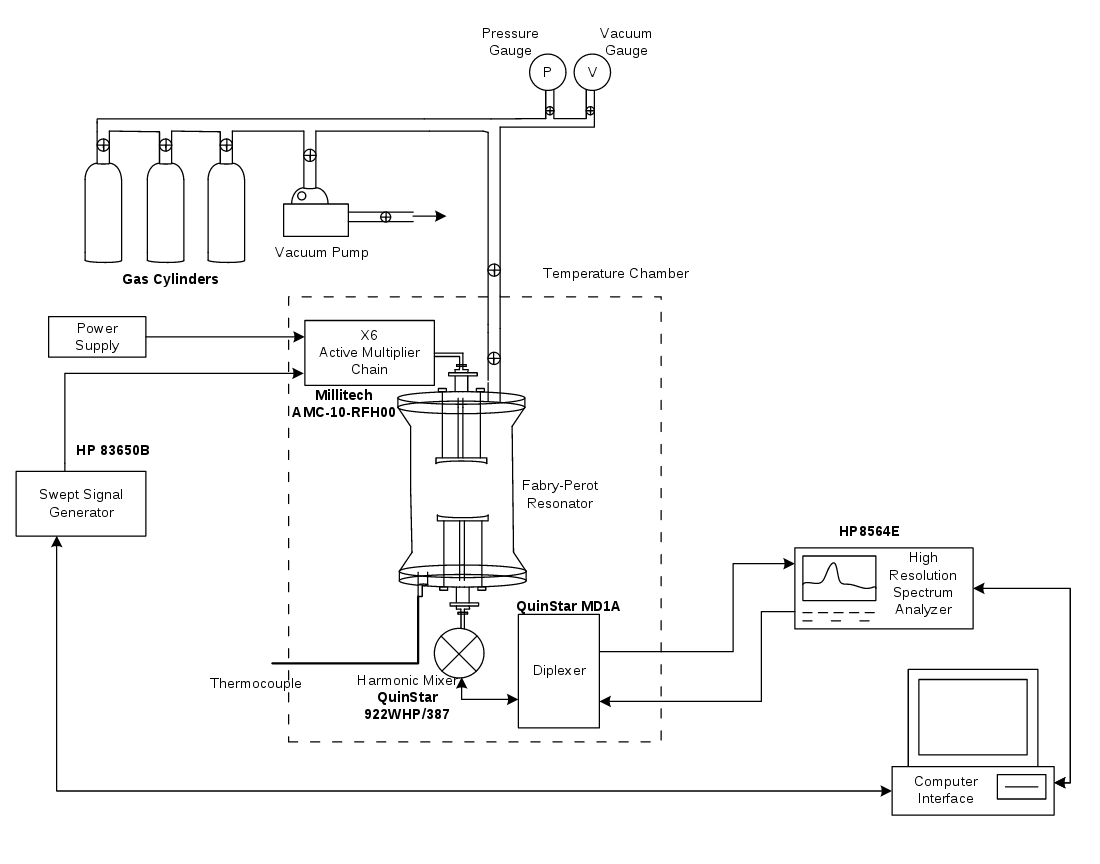
\includegraphics[width=0.7\textwidth]{./images/w-bandsystem.png}
	\caption{Block diagram of the W band measurement system. Solid lines represent the electrical connections and the arrows show the direction of the signal propagation. Valves controlling the flow of gasses are shown by small crossed circles.}
    \label{fig:wbandimage}
\end{figure}


\subsubsection{F-band Subsystem}
The F-band measurement system is used to measure the 2-3 mm-wavelength properties of sulfur dioxide and is shown in figure \ref{fig:fbandimage}.

The swept signal generator (HP 83650B) is used to generate a signal in the 33-50 GHz range which
is amplified and fed through a frequency tripler. The output of the tripler is fed to the input end of the FPR. The RF signal from the output port of the FPR is fed to a harmonic mixer which can operate with an LO frequency as high as 18 GHz. An external diplexer is used to combine the IF and LO signals. For a particular RF and IF frequency,  the LO frequency can be computed using

\begin{equation} \label{eq:fbandlo}
f_{LO} = \frac{f_{RF} - f_{IF}}{N_H	}
\end{equation}

\noindent where N$_H$ is the lowest integer such that $f_{lo} < 18 GHz$.

\begin{figure}[H]
    \centering
	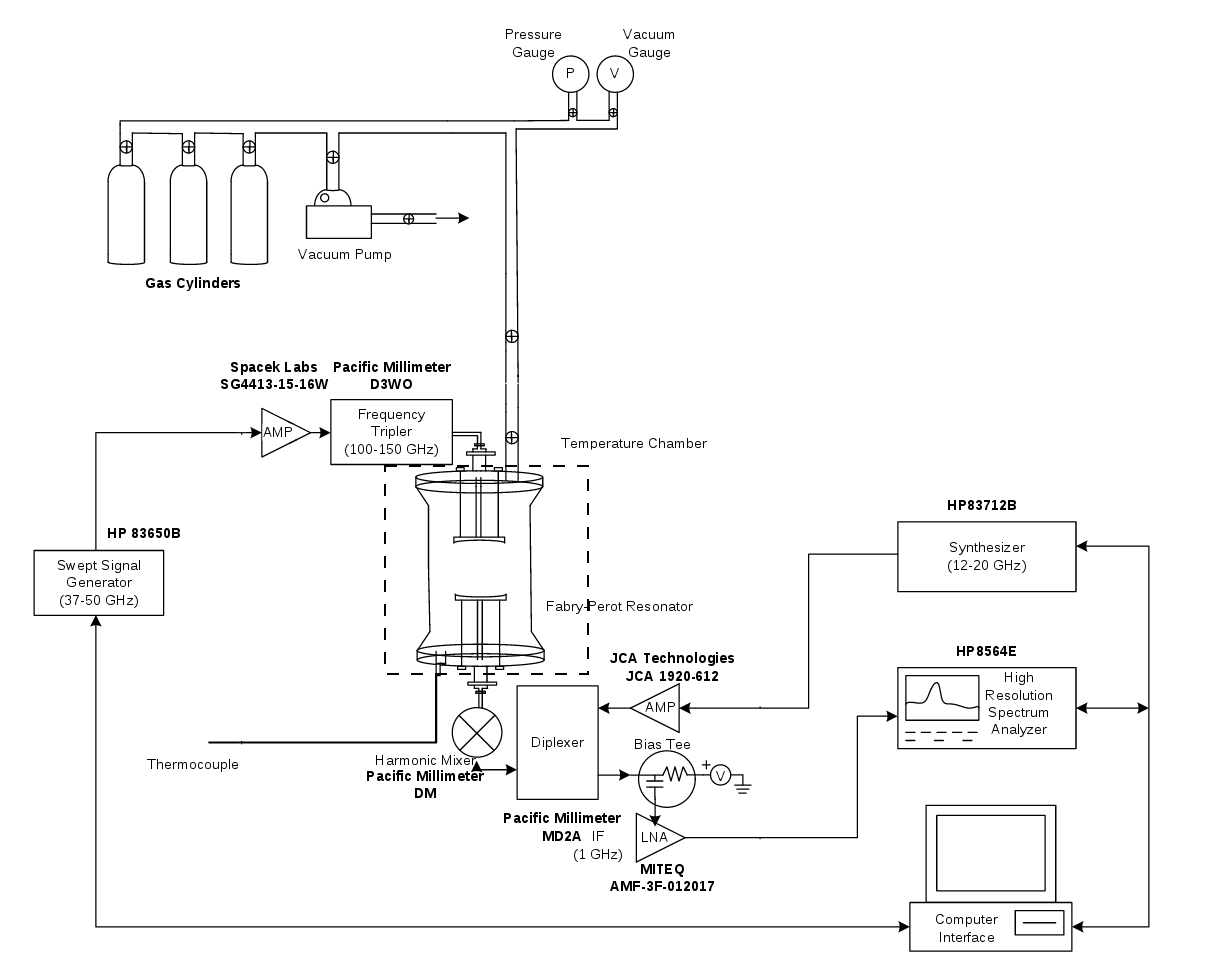
\includegraphics[width=0.7\textwidth]{./images/f-bandsystem.png}
	\caption{Block diagram of the F band measurement system. Solid lines represent the electrical connections and the arrows show the direction of the signal propagation. Valves controlling the flow of gasses are shown by small crossed circles.  }
    \label{fig:fbandimage}
\end{figure}

\subsection{Data Handling Subsystem}

The data acquisition system consists of a computer connected to the spectrum analyzer (HP 8564E), swept signal generator (HP 83650B), and continuous wave (CW) signal generator (HP 83712B, the local oscillator for the F-Band system) via a general purpose interface bus (GPIB). The instruments are controlled via Matlab script and their appropriate programming language. The software used is similar to Devaraj and Steffes \cite{system-description} \cite{Devaraj-thesis} with modifications for equipment changes.

\subsection{Measurement Procedure}

The most important prerequisite for performing measurement of gas properties is ensuring a leak-proof system. This is done through two methods, the first is by drawing a vacuum inside the FPR and verifying the integrity of the vacuum over time. The second way is by adding a positive pressure of CO$_2$ to the system and making sure there are no leaks in any of the connectors and valves. Ensuring a leak-proof system allows for not only precise measurements but also ensures no toxic gases are released into the testing environment.

After the system is ensured to be leak-proof and at a stable temperature, a vacuum is drawn and a measurement is taken using the appropriate subsystem (W-band for 3-4 mm-wavelengths, F-band for 2-3 mm-wavelengths). This allows for a base line measurement of the FPR's resonances and the Quality factor. Once this baseline is established the gas under test is added to the system.

Once the gas temperature has stabilized, another set of tests measuring the resonant frequencies along with the quality factors is taken. More gas is added and the procedure is repeated until all suitable pressures are taken. A vacuum is drawn once again but this time it is pumped overnight due to the gas being tested (SO$_2$) and its properties of ``sticking'' (or adsorbing) to metal. Another vacuum measurement is taken to measure any possible system error.

Once the second vacuum measurements are taken CO$_2$ is then added to the chamber until the resonances are matched to the same frequency of our test gas. Again measurements are taken and this is repeated for every pressure of the test gas. Once this is finished a vacuum is again drawn and another test is taken. 

Lastly the system is set up for a transmissivity test where we measure t (equation \ref{eq:t}) for each given resonant frequency. The system is then set back up and is ready for a new test. Reference table \ref{tab:testmatrix} for the testing matrix being used.

\subsection{Measurement Uncertainties}


\subsubsection{Absorptivity}

There are five uncertainties for any absorptivity measurements using the millimeter wavelength system: instrumentation errors and electrical noise ($Err_{inst}$), errors in dielectric matching ($Err_{diel}$), errors in transitivity measurement ($Err_{trans}$), errors due to resonance asymmetry ($Err_{asym}$), and errors in measurement conditions ($Err_{cond}$) resulting from uncertainties in temperature, pressure, and mixing ratio. The term $Err$ is used for representing uncertainties instead of the more frequently used $\sigma$ to avoid confusion between $1\sigma$,$2\sigma$, and $3\sigma$ uncertainties.

Instrumental errors and electrical noise are caused due to the sensitivity of the electrical devices and their ability to accurately measure bandwidth ($BW_{measured}$) and the center frequency ($f_o$). Electrical noise arises from the frequency references and the noise of the internal electronics. Since electrical noise is uncorrelated, it's best estimate of the uncertainty is the mean of multiple measurements. The variance of the best error estimate is given by the sample variance ($S^2_N$) weighted by the confidence coefficient ($B$) as
\begin{equation}\label{eq:sigman}
\sigma^2_N = B \frac{S^2_N}{N_{samples}}
\end{equation}

\noindent where $N_{samples}$ is the number of independent measurements of the sample. For the millimeter-wavelength system, five sets of independent measurements of each resonance are taken. A confidence coefficient ($B$) of 2.776 is used. This corresponds to the 95\% confidence interval. The center frequency standard deviation is very small and its effect on the uncertainty in $Q$ is negligible. Therefore, $S_N$ i the sample standard deviation of the bandwidth of the measurements.

The HP 8564E spectrum analyzer is used for measuring the resonances in the millmeter-wavelength system. It's manufacturer specified instrumental uncertainties are the $3\sigma$ values \cite{Hewlett-Packard}. The $3\sigma$ standard deviation for the center frequency and bandwidth are estimated by 

\begin{equation}\label{eq:sigmao}
Err_o \leq \pm (f_o \times f_{ref\:acc} + 0.05 \times SPAN + 0.15 \times RBW +10 ) (Hz)
\end{equation}
\begin{equation}\label{eq:sigmabw}
Err_{BW} \leq \pm (BW_{measured} \times f_{ref\;acc} + 4 \times N_H +2 \times LSD ) (Hz)
\end{equation}

\noindent where $f_{ref\;acc}$ is given as

\begin{equation}\label{eq:frefacclong}
\begin{split}
f_{ref\;acc} = (aging \times {time\;since\;calibration}) + {inital\;achievable\;accuracy} \\
+ {temperature\;stability}
\end{split}
\end{equation}

\noindent and $f_o$, SPAN, RBW, $N_H$, and LSD are the center frequency, frequency span, resolution bandwidth, harmonic number, and least significant digit of the bandwidth measurement, respectively. LSD is calculated as $LSD = 10^x$ for the smallest positive integer value of x such that SPAN $< 10^{x+4}$. For SPAN $\leq 2$ MHz$\times N_h$, the SPAN multiplication factor of 0.05 is replaced with 0.01. For the spectrum analyzer used, $f_{ref\;acc}$ reduces to

\begin{equation}\label{eq:frefacc}
f_{ref\;acc} = (10^{-7} \times {years\;since\;calibrated}) + 3.2\times 10^{-8}
\end{equation}

The worst case scenario is used to transform the uncertainty in center frequency and bandwidth for both loaded and dielectrically matched measurements into an uncertainty in absorptivity as described in DeBoer and Steffes \cite{DeBoer-Steffes}.

\begin{equation}
Err^2_\Psi = \langle {F_l^2}\rangle + \langle {F_m^2}\rangle -\langle {F_l F_m}\rangle
\end{equation}

\noindent where
\begin{equation}
\langle {F_i^2}\rangle = \frac{\Upsilon_i^2}{f_{oi}^2}
\left[ \frac{Err_o^2}{Q_l^2} + Err_{BW}^2 + Err_{Ni}^2 + \frac{2Err_o Err_{BW}}{Q_i} \right], i= l,m
\end{equation}
\begin{equation}
\langle {F_l F_m}\rangle = -\frac{\Upsilon_l \Upsilon_m}{f_{ol} f_{om}}
\left[ \frac{Err_o^2}{Q_i Q_m} + Err_{BW}^2 + \frac{Err_o Err_{BW}}{Q_l} + \frac{Err_o Err_{BW}}{Q_m}\right]
\end{equation}
\begin{equation}
Q_i = \frac{f_{oi}}{f_{BWi}}, i = l,m
\end{equation}
\begin{equation}
\Upsilon_i = 1- \sqrt{t}, i = l,m
\end{equation}
where $l,m$ denote loaded and dielectrically matched cases, respectively and $f_{ol,om}$ and $f_{BWl,BWm}$ represent center frequency and bandwidth of loaded and dielectrically matched cases respectively. The $2\sigma$ uncertainty of the measured gas absorption due to instrumental errors and electrical noise is given by
\begin{equation}
Err_{inst} = \pm \frac{8.686\pi}{\lambda}Err_\Psi\;(dB/km)
\end{equation}
where $\lambda$ is the wavelength in km. 

Errors in dielectric matching occur when the when the center frequency of the matched measurements are not precisely aligned with the center frequency of the loaded measurement. Since the Q of the resonator can vary slightly this causes an uncertainty in the Q of the matched measurement at the true center frequency of the loaded measurement. The method used to calculate the magnitude of this effect is similar to Devaraj \cite{Devaraj-thesis}. While this error is the most trivial due to the high precision of the software controlled matching it is important to calculate and account for.The magnitude of this effect is calculated by comparing the Q of the three vacuum measurements to that of the dielectric matched measurements

\begin{equation}
\left(\frac{dQ}{df} \right)_i = \left|\frac{Q_{vac,i} - Q_{matched,i}}{f_{vac,i} - f_{matched,i}} \right| \textnormal{ for } i = 1,2,3
\end{equation}

The maximum of the three values is used to calculate a $dQ$ value

\begin{equation}
dQ = \left(\frac{dQ}{df} \right)_{max} \times |f_{loaded} - f_{matched}|
\end{equation}
where $f_{loaded}$ and $ f_{matched}$ are the center frequencies of the resonances under loaded and matched conditions. The error in absorbtivity due to imperfect dielectric matching is then computed by propagating $\pm dQ$ through Equation \ref{eq:alphamatch}.
% \times \left| \left( \frac{1-\sqrt{t_{loaded}}}{Q^m_{loaded}} - \frac{1-\sqrt{t_{matched}}}{Q^m_{matched} + dQ} \right) \left|
\begin{equation}
\begin{split}
Err_{diel} &= \frac{8.686 \pi}{\lambda} 
\\ &\times \left| \left( \frac{1-\sqrt{t_{loaded}}}{Q^m_{loaded}} - \frac{1-\sqrt{t_{matched}}}{Q^m_{matched} + dQ} \right) - \left( \frac{1-\sqrt{t_{loaded}}}{Q^m_{loaded}} - \frac{1-\sqrt{t_{matched}}}{Q^m_{matched} - dQ} \right) \right|\\
 &(dB/km)
\end{split}
\end{equation}

Transmissivity errors are due to the uncertainties in the measurement amplitude. This is caused by loss in the millimeter-wavelength instruments (signal generators and spectrum analyzer), cables, adapters, and waveguides used in this system. Measuring this is done taking multiple tests of the system without the FPR and finding the standard deviation ($S_N$) and weighing it by it's confidence coefficient
\begin{equation}
Err_{msl} = \frac{4.303}{\sqrt{3}}S_N
\end{equation}

For the millimeter-wavelength system, the signal level measurements involve sampling the RF power with a WR-10 20 dB directional coupler to feed the harmonic mixer for down-conversion and detection. While this ensures that the input to the harmonic mixer does not exceed its maximum allowed input power of -10 dBm, the WR-10 does not uniformly sample the input signal throughout the entire frequency range. To compensate for this an aditional 1.5 dB uncertainty is added to insertion loss error. The signal generator has a temperature stability of 1 dB/$10^\circ$ C, but an internal temperature equilibrium is reached after two hours \cite{Hewlett-Packard}. Since the measurements units are stored at a constant temperature this uncertainty can be disregarded. The total uncertainty in insertion loss for the millimeter-wavelength system is calculated by
\begin{equation}
Err_{ins\;loss} = Err_{msl} +1.5\;(dB)
\end{equation}

The error in insertion loss is used to compute the transissivity error
\begin{equation}
Err_{t,i} = \frac{1}{2} ( 10^{-S_i - Err_{ins\;loss}} - 10^{-S_i + Err_{ins\;loss}}) , i=l,m
\end{equation}
where l,m are the loaded and matched cases, respecivey, and S is the insertion loss of the resonator. This is used to compute the $2\sigma$ uncertainties in opacity and is expressed as
\begin{equation}
\begin{split}
Err_{trans} &= \frac{8.686 \pi}{2\lambda}\\ 
 &\times \left| \left( \frac{\sqrt{t_l + Err_{t,l}}- \sqrt{t_l - Err_{t,l}}}{Q^m_{loaded}} - \frac{\sqrt{t_m - Err_{t,m}}- \sqrt{t_m + Err_{t,m}}}{Q^m_{matched}} \right) \right|\\
 &(dB/km).
\end{split}
\end{equation}

Errors from asymmetry are due to the asymmetric nature of the resonances. These are more prominent at low temperatures and short wavelength. Errors due the asymmetry results from the disproportionate asymmetric broadening of the loaded measurements compared to the matched measurements. Equivalent full bandwidths based on assuming symmetry of the high and low sides of the resonances are calculated as
\begin{equation}
BW_{high} = 2 \times (f_{high} - f_{center})
\end{equation}
\begin{equation}
BW_{low} = 2 \times (f_{center} - f_{low})
\end{equation}
where $BW_{high}, BW_{low}, f_{high}, f_{center}$, and $f_{low}$ are the high bandwidth, low bandwidth, higher frequency half power point, center frequency, and lower frequency half power point, respectively. The difference between the opacities calculated using $BW_{high}$ and $BW_{low}$ is defined as $Err_{asym}$ and is calculated by
\begin{equation}
\begin{split}
Err_{asym} &= \frac{8.686 \pi}{\lambda} 
\\ &\times \left| \left( \frac{1-\sqrt{t_{loaded}}}{Q^m_{loaded,high}} - \frac{1-\sqrt{t_{matched}}}{Q^m_{matched,high}} \right) - \left( \frac{1-\sqrt{t_{loaded}}}{Q^m_{loaded,low}} - \frac{1-\sqrt{t_{matched}}}{Q^m_{matched,low}} \right) \right|\\
 &(dB/km)
\end{split}
\end{equation}
Where $Q^m_{matched,high/low}$ and $Q^m_{loaded,high/low}$ are the measured Qs evaluated using the high and low bandwidths for loaded and matched cases. 

The measured uncertainties in temperature, pressure, and concentration contribute to the total uncertainties due to the measurement conditions ($Err_{cond}$). While this does not affect the measurements it still needs to be accounted for during the creation of the models for opacity based on experimental data. It is computed by
\begin{equation}
Err_{cond} = \sqrt{Err_{temp}^2 + Err_{p}^2 + Err_{c}^2} (dB/km)
\end{equation}
with $Err_{temp}^2, Err_{p}^2 $, and $ Err_{c}^2$ representing the 2$\sigma$ uncertainties in the proposed opacity model corresponding to the uncertainties in temperature, pressure, and concentration. 

Measuring temperature was done using a T type thermocoupler along with a Wavetek 23XT voltmeter. The voltmeter has a temperature accuracy of $\pm (1\% + 2^\circ C)$. Since the voltmeter has a Cold Compensation circuitry it is unnecessary to modify the temperature read from ambient. Also since a test takes an hour to run the temperature drift is insignificant. The uncertainty in temperature reading is calculated by
\begin{equation}
T = T_{read} \pm ( T_{read} \times 1\% + 2)
\end{equation}
Where $T_{read}$ is the temperature readout from the Voltmeter.

Pressure was measured using an Omega DPG-7000 which has an accuracy of $\pm 0.05\%$. Since this pressure gauge measures pressure relative to ambient it is necessary to take a measurement before and after each test. The average change in pressure during a test was at most 2 mbar. The way a vacuum was measured was by comparing the Omega DPG-7000 reading to that of an absolute pressure gauge (Druck DPI 104). The Druck has an accuracy of $\pm 0.05\%$ as well but a resolution of $\pm 1$ mbar. The uncertainty in pressure reading is calculated by
\begin{equation}
P = P_{read} \pm ( P_{read} \times .05\% + 3)
\end{equation}
Where $P_{read}$ is the pressure read from the Omega DPG-7000.

Since $Err_{cond}$ is dependent on the opacity model, this uncertainty is maintained separately from $Err_{tot}$. Thus the total 95\% confidence for the measurement uncertainty is expressed in dB\/km as per Hanley \cite{Hanley-thesis}
\begin{equation}
Err_{tot} = \sqrt{Err_n^2 + Err_{diel}^2 + Err_{trans}^2 + Err_{asym}^2} \;(dB/km).
\end{equation}